%Beamer class
\documentclass{beamer}

\usepackage[czech]{babel}
\usepackage[cp1250]{inputenc}
\usepackage{fontenc}
\usepackage{tgheros}
\usepackage{array}
\usepackage{color}
\usepackage{hyperref}

\usetheme{Antibes}
\usecolortheme{crane}


\title[BE1M13VES]{BE1M13VES}
\subtitle[Manufacturing of Electrical Components] {Manufacturing of Electrical Components}
\author[Brejcha]{Michal Brejcha}
\institute[CTU]{CTU in Prague}
\date[Prague, 2017]{Prague, 2017}

\begin{document}
%------------------------------------------------------------------------------
%Uvodni slajd
%------------------------------------------------------------------------------
\frame{\titlepage}

\begin{frame}
\frametitle{Overview} 
\tableofcontents
\end{frame}

\AtBeginSection[]
{
  \begin{frame}
    \frametitle{TOPIC}
    \tableofcontents[currentsection]
  \end{frame}
}

%------------------------------------------------------------------------------
%Variable Resistors
%------------------------------------------------------------------------------
\section{\texorpdfstring{Variable Resistors}{Resistance value}}
%------------------------------------------------------------------------------
	\begin{frame}
    \frametitle{Variable resistors}
		\begin{center}
		\begin{tabular}{p{0.12\linewidth} p{0.78\linewidth}}
			\textbf{Types:} 					& 
			\begin{itemize}
				\item potentiometers (for controls - a lot of cycles),
				\item trimmers (for settings - a few of cycles).
			\end{itemize}
		\end{tabular}
		\end{center}
		
		\begin{itemize}
			\item Design of variable resistors is based on slider (wiper) moving or rotating above a resistive track.
		\end{itemize}
		\begin{center}
		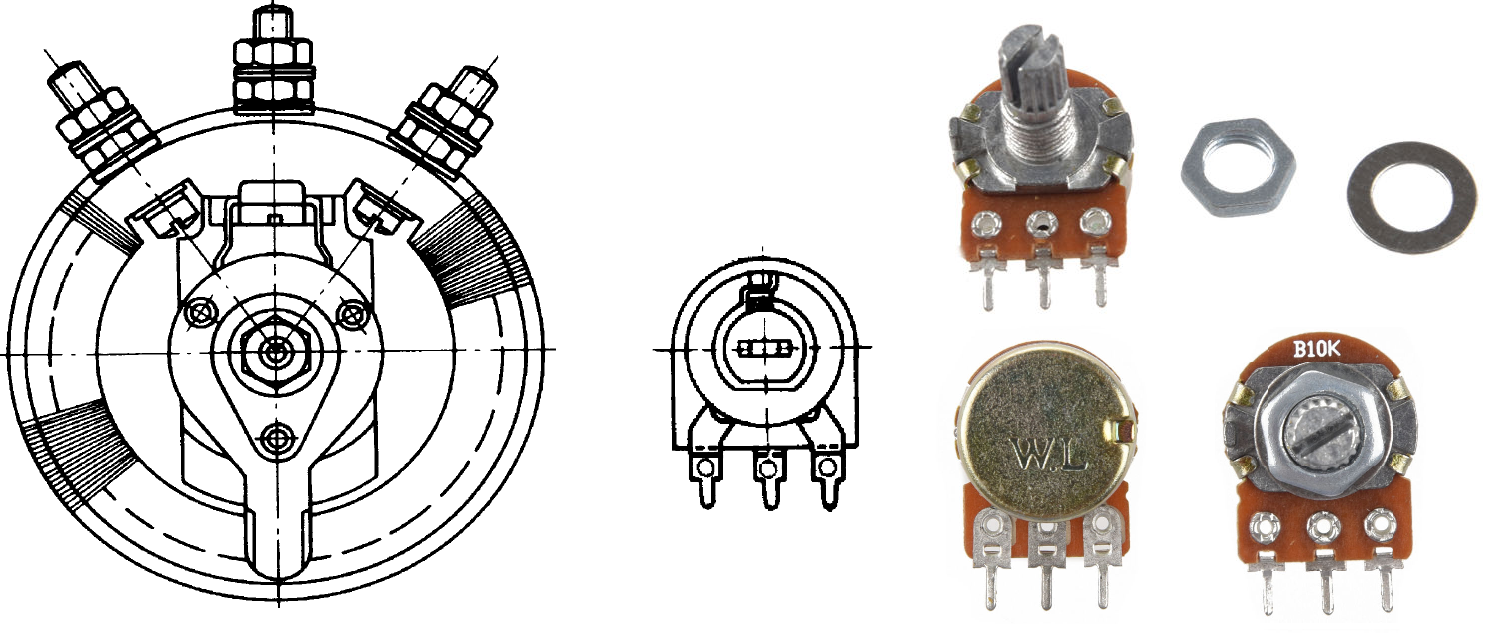
\includegraphics[scale=0.2]{obr01_potTrim.png}
		\end{center}
  \end{frame}
%------------------------------------------------------------------------------
	\begin{frame}
    \frametitle{Parameters}
		\begin{itemize}
			\item Similar parameters to normal resistors
			\item Values from sets E6 or E12
			\item Resistivity of layer tracks can be between 100~$\Omega$ and 5~M$\Omega$
			\item Resistivity of wired tracks can be between 1~$\Omega$ and 100~k$\Omega$
			\item Common tolerance (accuracy) is 20~$\%$, in case of special usage 0.3~$\%$,
			\item Several constructions:
		\end{itemize}
		\begin{center}
		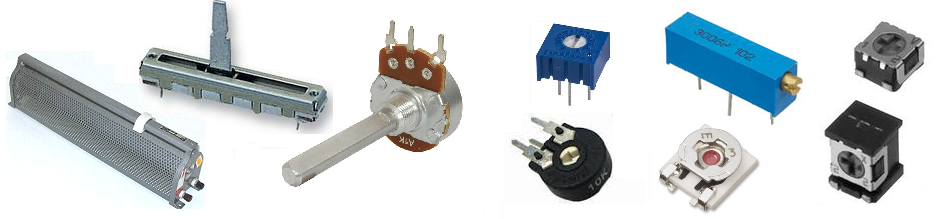
\includegraphics[scale=0.35]{obr04_konstrukce.png}
		\end{center}
  \end{frame}
%------------------------------------------------------------------------------
	\begin{frame}
    \frametitle{Disassembly}
		\begin{center}
		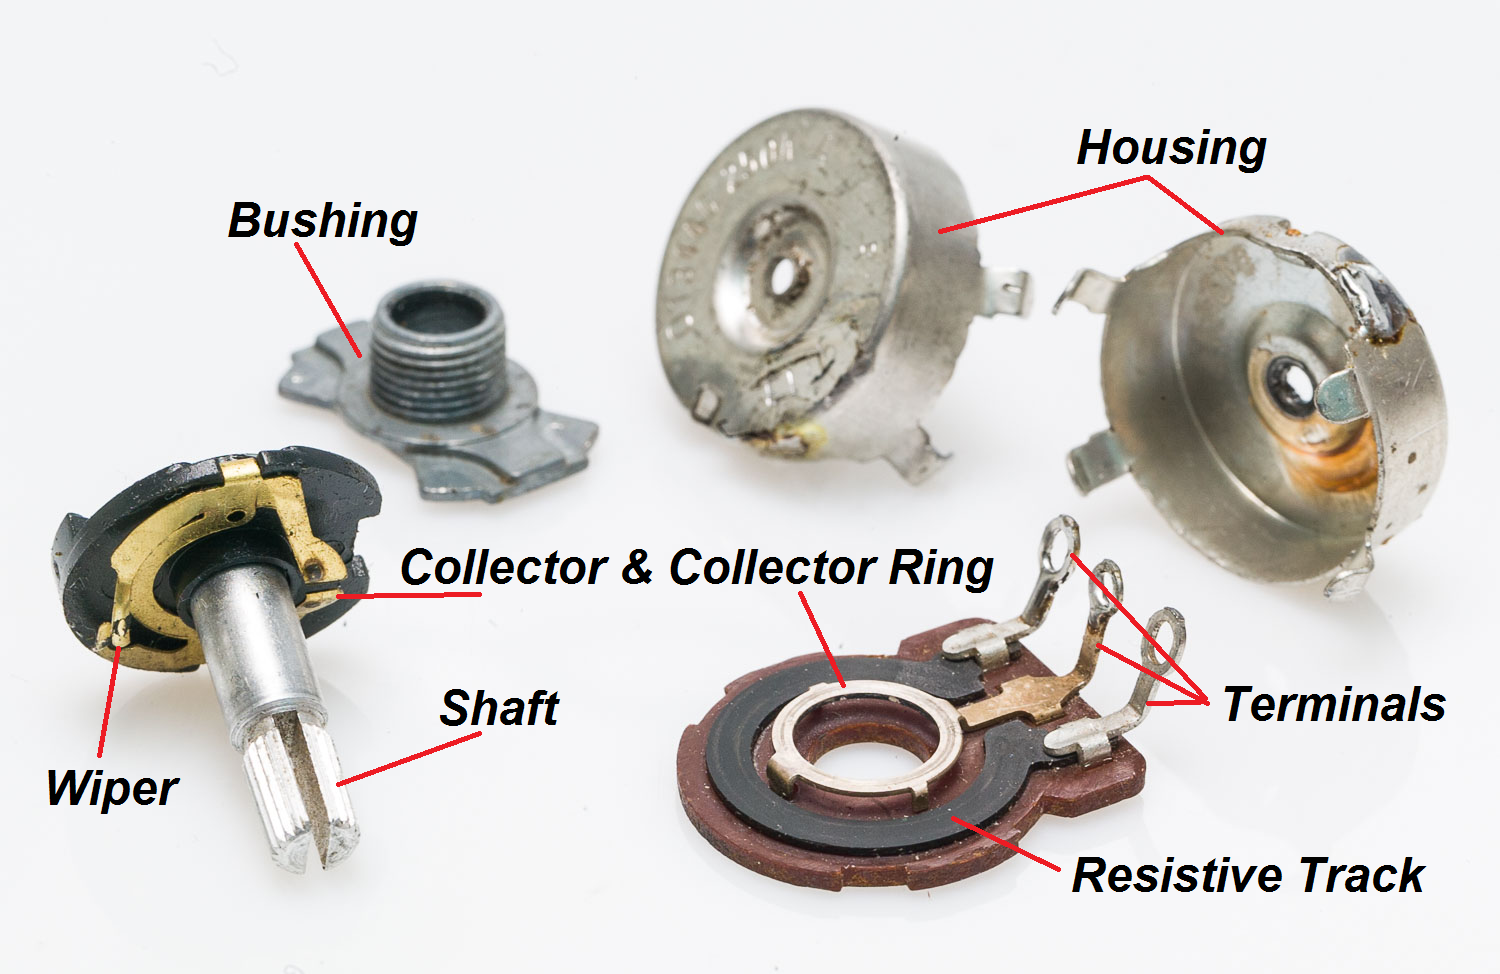
\includegraphics[scale=0.25]{obr03_rozebrany.png}
		\end{center}

  \end{frame}
%------------------------------------------------------------------------------
	\begin{frame}
    \frametitle{Technology}
		\small
		\begin{center}
		\begin{tabular}{p{0.25\linewidth} p{0.65\linewidth}}
			\textbf{Track:} 					& wire, varnished ceramic, conductive plastic (carbon), cermets (ceramics + metal)\\
			\textbf{Wiper:} 					& metal or with carbon layer, small transient resistivity is required\\
			\textbf{Track Profile:} 	& linear, logarithmic, exponencial\\
		\end{tabular}
		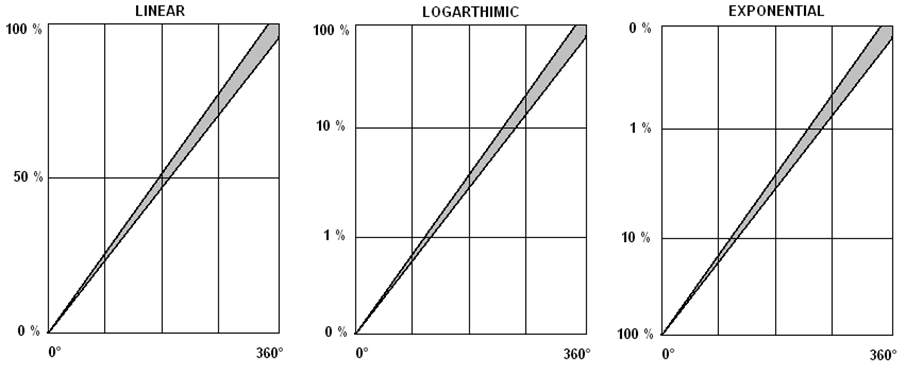
\includegraphics[scale=0.4]{obr02_profily.png}
		\end{center}

  \end{frame}
%------------------------------------------------------------------------------
	\begin{frame}
    \frametitle{Design of Resistive Track}
		Nonlinear resistive track is made from several layers.
		\begin{center}
		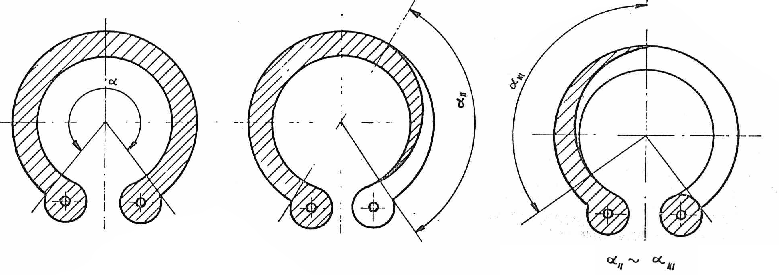
\includegraphics[scale=0.4]{obr05_vrstvyRDrahy.png}
		\end{center}
		\begin{itemize}
			\item The first layer is applied on an insulating pad, other layers are made on the previous one.
			\item Bottom layer has the highest resistivity, the top layer has the lowest resistivity.
		\end{itemize}
  \end{frame}
%------------------------------------------------------------------------------
	\begin{frame}
    \frametitle{Multiturn Potentiometers - ARIPOT and similars}
		\begin{center}
		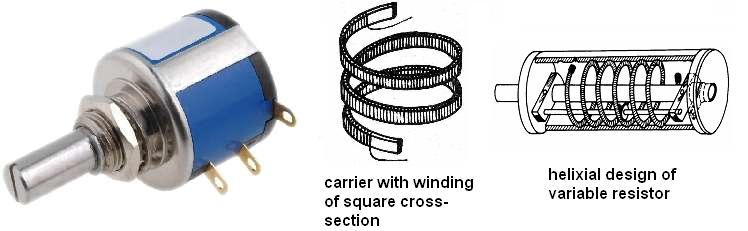
\includegraphics[scale=0.4]{obr06_viceotackovy.png}
		\end{center}
		\begin{itemize}
			\item Collector moves along helix winding or resistive track.
			\item The track can be long in comparison to common flat design.
			\item Collector must be able of axial movement - very precise construction, wiper in form of a roller.
		\end{itemize}
  \end{frame}
%------------------------------------------------------------------------------
	\begin{frame}
    \frametitle{Layers Overview}
		\begin{flushleft}
		\textbf{Varnished Track:} layer is sprayed or print via screen from a mixture of varnish and carbon filler.
		\end{flushleft}
		\begin{flushleft}
		\textbf{Cermets Track:} resistive layer is made from burned paste on a ceramic basis. Layers are made by screen-printing technology (silk-screen printing). Only linear profile can be made.
		\end{flushleft}
		\begin{flushleft}
		\textbf{Tracks from conductive plastics:} tracks have a large cross-section area, they are abrasion-proof, also tracks with non-linear profile can be made.
		\end{flushleft}
  \end{frame}
%------------------------------------------------------------------------------
	\begin{frame}
    \frametitle{Trimmers}
		\begin{itemize}
			\item Basic principle is the same for potentiometers as for trimmers. 
			\item Trimmers usually don't have shaft and knob, setting in done manually by some tool (e.g. screwdriver).
			\item Design is simplified - without cover, trimmers used to be fixed by outlets (missing armature/chassis).
			\item Long-life operation is not expected, trimmers are used just for settings.
		\end{itemize}
		\begin{center}
			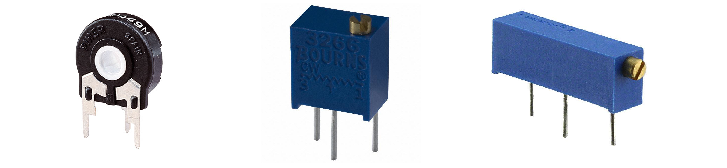
\includegraphics[scale=0.4]{obr07_trimry.png}
		\end{center}
  \end{frame}
%------------------------------------------------------------------------------
	\begin{frame}
    \frametitle{Comparison of different types of variable resistors}
		\tiny
		\begin{center}
		\begin{tabular}{|m{0.1\linewidth} | m{0.1\linewidth} | m{0.1\linewidth} | m{0.1\linewidth} | m{0.1\linewidth} | m{0.1\linewidth} | m{0.1\linewidth}|}
			\hline
			\hline
													& \textbf{carbon} & \textbf{cermets} & \textbf{wired} & \textbf{multiturn} & \textbf{plastic} & \textbf{cermets} \\
			\hline
			accuracy of track		& $10\%$ & $1\%$ & $1\%$ & $0.1\%$ & $10\%$ & $1\%$ \\
			\hline
			whisper signals			& $1$ $\mu$V/V & $10$ $\mu$V/V & none & none & $100$ $\mu$V/V & $100$ $\mu$V/V \\
			\hline
			max. power					& 1 W & 1 W & 1 kW & 1 W & 1 W & 2-3 W \\
			\hline
			life-time (cycles)	& $10^4-10^5$ & $10^4-10^5$ & $10^4-10^5$ & $10^7$ & $10^8$ & $100$ \\
			\hline
			stability						& $10\%$ & $1\%$ & $1\%$ & $0.1\%$ & $0.5\%$ & $1\%$ \\
			\hline
			\hline
		\end{tabular}
		\end{center}
  \end{frame}
%------------------------------------------------------------------------------
%Thermistors
%------------------------------------------------------------------------------
\section{\texorpdfstring{Nonlinear Resistors}{Nonlinear Resistors}}
%------------------------------------------------------------------------------
	\begin{frame}
    \frametitle{Nonlinear Resistors}
		\begin{itemize}
			\item thermistors (NTC, PTC). 
			\item voltage depended resistors (VDR) - varistors.
			\item photoresistors.
		\end{itemize}
  \end{frame}
%------------------------------------------------------------------------------
	\begin{frame}
    \frametitle{NTC Thermistor}
		\textbf{NTC} $=$ negative temperature coefficient
		$$R=A\cdot e^\frac{B}{T}$$
		\begin{tabular}{m{0.5\linewidth} m{0.4\linewidth}}
			\begin{itemize}
				\item A... Resistivity for infinity temperature
				\item B... Material parameter
				\item T... Thermodynamic temperature
			\end{itemize} & 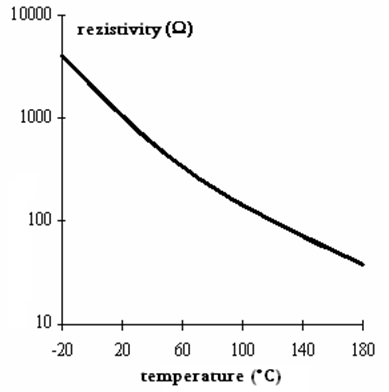
\includegraphics[scale=0.4]{obr08_zavislostNaTep.png}
		\end{tabular}
  \end{frame}
%------------------------------------------------------------------------------
	\begin{frame}
    \frametitle{NTC Thermistor}
		\begin{flushleft}
		\textbf{Parameters A, B}
		$$ln(R)=ln(A) + \frac{B}{T}$$
		This is a linear function of $ln(R)$ in dependency to $\frac{1}{T}$
		\end{flushleft}
		\begin{flushleft}
		\textbf{VA - characteristic:} affected by self heating.
		\begin{center}
		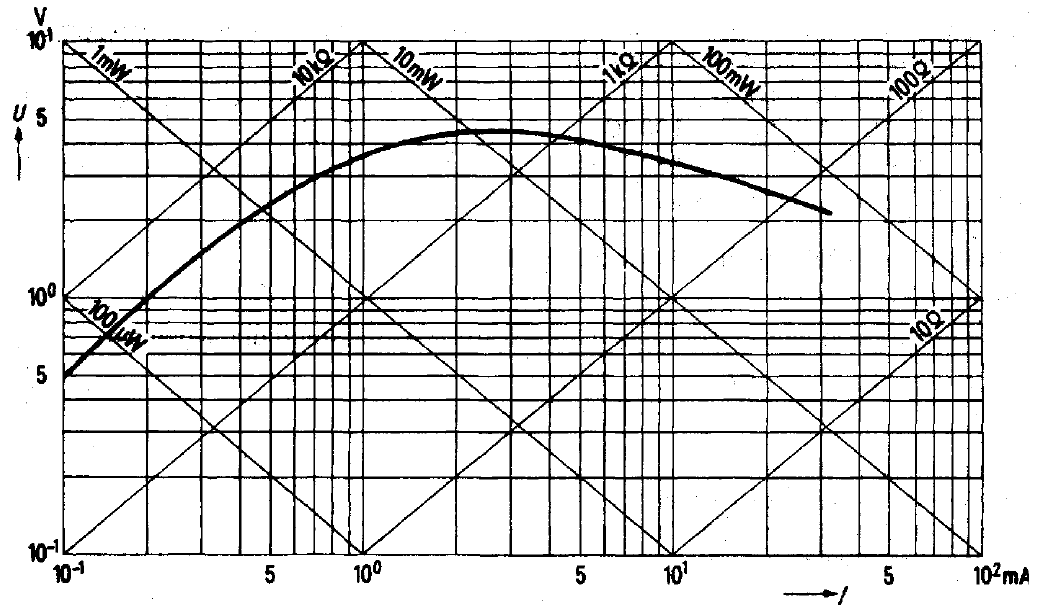
\includegraphics[scale=0.25]{obr09_vaNTC.png}
		\end{center}
		\end{flushleft}
  \end{frame}
%------------------------------------------------------------------------------
	\begin{frame}
    \frametitle{Packages Examples}
		\begin{center}
		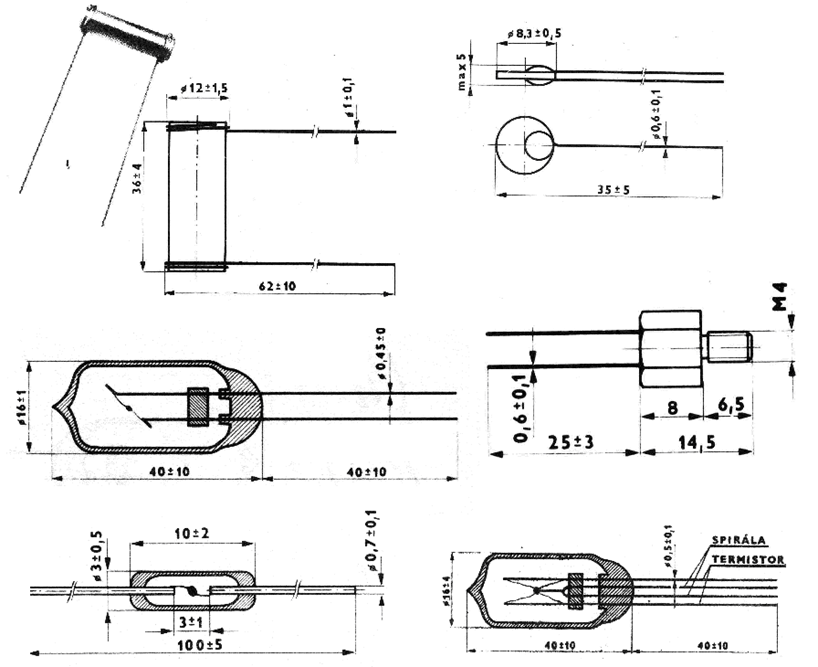
\includegraphics[scale=0.38]{obr10_prikladyNTC.png}
		\end{center}
  \end{frame}
%------------------------------------------------------------------------------
	\begin{frame}
    \frametitle{Design of NTC Thermistors}
		\small
		\begin{itemize}
			\item shapes similar to: pales, tablets, small pearls,
			\item materials: polycrystalline semiconductors plus oxides of $Mn$, $Ni$, $Cu$, $Co$, $Cr$, $Ti$, $W$, (in the past often used $UO_2$, $TiO_2$, $CuO$). Minced mixture of oxides must be homogenous and well mixed.
		\end{itemize}
		\textbf{Pales and tablets:}
		\begin{itemize}
			\item pressed under big stress (600 kg/cm$^2$) into required shapes,
			\item burning at temperature 1000 $^\circ$C (up to 1400 $^\circ$C) in oxidation atmosphere,
			\item soldering of $Cu$ outlets by $Ag$ paste.
		\end{itemize}
  \end{frame}
%------------------------------------------------------------------------------
	\begin{frame}
    \frametitle{Design of NTC Thermistors}
		\small
		\textbf{Small pearls:}
		\begin{itemize}
			\item between two wires of Pt-alloy (with diameter $25 - 100$ $\mu$m) is putted a drop of minced mixture,
			\item burning at temperature 1000 $^\circ$C (up to 1400 $^\circ$C),
			\item encapsulation into glass (thermometers) or vacuum capsule,
			\item important is artificial aging to stabilizing electric features.
		\end{itemize}
  \end{frame}
%------------------------------------------------------------------------------
	\begin{frame}
    \frametitle{PTC Thermistors}
		\textbf{PTC} $=$ positive temperature coefficient, at cold-state low impedance, at hot-state high impedance. This effect is caused by ferroelectric material and changes of its permittivity.
		\small
		\begin{tabular}{m{0.55\linewidth} m{0.35\linewidth}}
			\begin{itemize}
				\item \textbf{low temperature} $=$ ferroelectric domains exhibit high electrical strength - conductive low impedance state,
				\item \textbf{high temperature} $=$ ferroelectric domains exhibit lower permittivity and lower electric strength - high impedance state.
				\item \textbf{PTC} are both voltage and frequency dependent devices.
			\end{itemize} & 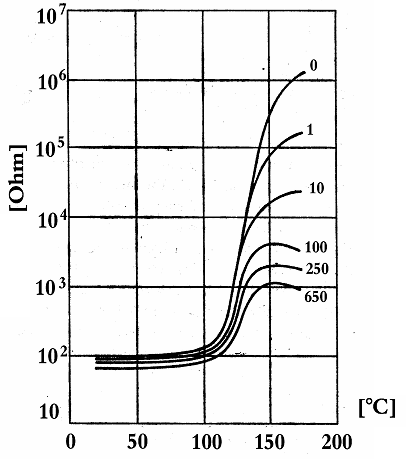
\includegraphics[scale=0.4]{obr11_zavislostNaTepPTC.png}
		\end{tabular}
  \end{frame}
%------------------------------------------------------------------------------
	\begin{frame}
    \frametitle{Design of PTC Thermistors}
		\begin{itemize}
			\item used shapes: pales and tables again,
			\item materials: burned mixture of $BaCO_3$, $SrCO_3$, $La_2O_3$, $TiO_2$, $SiO_2$,
			\item processing: minced mixture is formed under a big stress; burning at the temperature 1100 $^\circ$C starts calcinations process; than second mincing and final burning/annealing at 1400 $^\circ$C for 2 hours; soldering of $Cu$ outlets (wires).
		\end{itemize}
		\begin{center}
			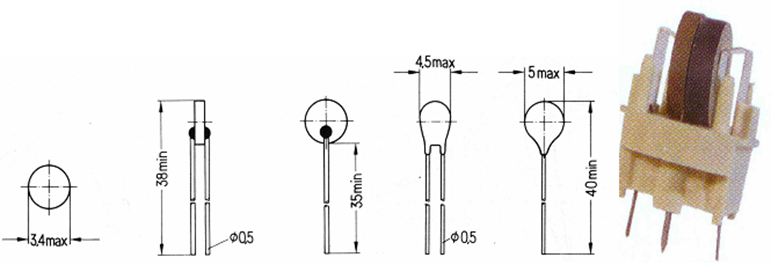
\includegraphics[scale=0.4]{obr12_prikladyPTC.png}
		\end{center}
  \end{frame}
%------------------------------------------------------------------------------
	\begin{frame}
    \frametitle{Varistors}
		\begin{center}
			\begin{tabular}{m{0.6\linewidth} m{0.3\linewidth}}
			\small
			
			\begin{itemize}
				\item B... Material parameter
				\item resistor made from polycrystalline semiconductor,
				\item fast increase of flowing current after achieving of breakdown voltage,
				\item decrease of impedance is caused by increase of electrical strength between domains of semiconductor,
				\item fast response in the order of 50 ns,
				\item at higher frequencies VDR behaves as capacitor with big power loss.
			\end{itemize} & $$I= B\cdot V^\alpha$$ 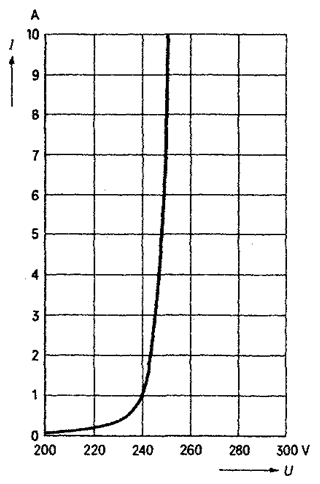
\includegraphics[scale=0.4]{obr13_vaVaristor.png}
		\end{tabular}
		\end{center}
  \end{frame}
%------------------------------------------------------------------------------
	\begin{frame}
    \frametitle{Design of Varistor}
			\begin{center}
			\begin{tabular}{m{0.5\linewidth} m{0.35\linewidth}}
			\small
			\begin{itemize}
				\item shape: typically tablets, pressed from a mixture of polycrystalline semiconductor,
				\item material: $SiC$ (old), now $ZnO$ with $MnO$, $Sb_2O$, $MgO$, $Bi_2O_3$ and fixed with a glass fibers,
				\item outlets: burned $AgPd$ pads and soldered $Cu$ wires outlets,
				\item covering: synthetic or epoxy resin.
			\end{itemize} & 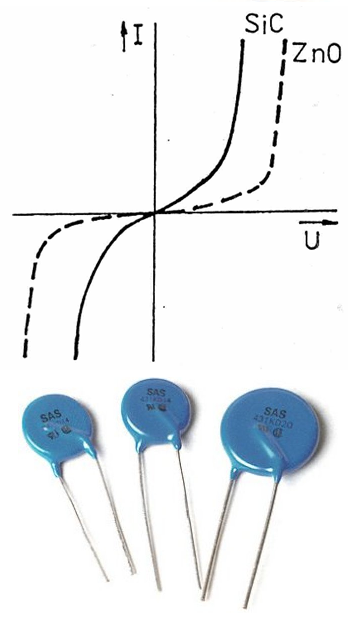
\includegraphics[scale=0.4]{obr15_varPouzdra.png}
		\end{tabular}
		\end{center}
  \end{frame}
%------------------------------------------------------------------------------
\end{document}